% !TeX program = xelatex
% Build with: tectonic ProphetMatching.tex
\documentclass[11pt,a4paper]{article}
\usepackage[T1]{fontenc}
\usepackage[english]{babel}
\usepackage{lmodern,amsmath,amssymb,booktabs,array,geometry,tikz}
\usepackage{hyperref}
\geometry{margin=25mm}
\definecolor{tinta}{gray}{0}
\definecolor{rara}{gray}{0}
\hypersetup{colorlinks=true,linkcolor=blue,urlcolor=blue,citecolor=blue,
 pdfauthor={GPT-6.2 Astra; Raimundo Olmos Rodríguez},
 pdftitle={An Upper Bound for Prophet Matching under Adversarial Edge Arrivals},
 pdfsubject={AI-generated research note with a finite witness and a Lean 4 certificate},pdflang={en}}
\urlstyle{same}
\setlength{\parindent}{17pt}
\setlength{\parskip}{0pt plus 1pt}
\setlength{\emergencystretch}{1.5em}
\newcommand{\E}{\mathbb{E}}
\newcommand{\OPT}{\mathrm{OPT}}
\newcommand{\numon}{25\,600\,000\,000}
\newcommand{\numoff}{61\,762\,963\,837}
\newcommand{\masa}{320\,000\,000}
\renewcommand{\refname}{References}
\newtheorem{teorema}{Theorem}
\newtheorem{lema}{Lemma}
\newenvironment{prueba}[1][Proof]{\par\smallskip\noindent\textit{#1.}\enspace}{\unskip\nobreak\hfill\(\square\)\par\smallskip}
\newcommand{\ON}{\mathrm{ON}}
\newcommand{\F}{\mathcal F}
\title{An Upper Bound for Prophet Matching\\[.35em]
under Adversarial Edge Arrivals}

\author{GPT-6.2 Astra \and Raimundo Olmos Rodríguez}
\date{November 25, 2026}
\begin{document}
\maketitle
\begin{abstract}
In prophet matching, an online policy observes independent edge weights one at a time and makes irrevocable decisions subject to the matching constraint. Under adversarial edge arrivals, the optimal competitive ratio is at most \(\numon/\numoff=0.414487880917\ldots\), even when the policy knows the arrival order and has access to private randomness. This improves the upper bound of \(0.418928\) proved by Soto and Verdugo. The witness is a simple graph on six vertices with seven edges. Conditioning on the first acceptance determines the optimal online value. Enumerating eight states gives the expected weight of the maximum integral matching. A Lean~4 certificate accompanies the finite instance and the exact calculations.
\end{abstract}
\noindent\textbf{Keywords.} Prophet inequalities, maximum-weight matching, online algorithms, competitive analysis.

\medskip\noindent\textbf{AI use and contributions.} GPT-6.2 Astra, used through OpenAI Codex, generated the construction, mathematical argument, Lean code, literature search, and manuscripts in Spanish and English. Raimundo Olmos Rodríguez posed the research question, requested verification and revisions, and shared the materials. Lean checked the supplied formal statements. Independent expert review and confirmation of priority remain open.
\tableofcontents
\clearpage
\section{Model and main result}\label{sec:modelo}
An instance \(I\) consists of a finite simple graph \(G=(V,E)\), an ordering \(e_1,\ldots,e_m\) of its edges, and independent, nonnegative, integrable random weights \(W_1,\ldots,W_m\). The order is fixed before the weights are drawn. Write \(\mathcal M(G)\) for the subsets of \(E\) whose edges are pairwise vertex-disjoint. The prophet's payoff is the random variable
\[
  \OPT(I)=\max_{M\in\mathcal M(G)}\sum_{i:\,e_i\in M} W_i .
\]

The policy knows the graph, the order, and the distributions in advance. Let \(U\) be its private random seed, independent of the weights, and let \(\F_i=\sigma(U,W_1,\ldots,W_i)\) be the information available when \(e_i\) arrives. An admissible policy \(\pi\) chooses an \(\F_i\)-measurable acceptance indicator \(A_i\in\{0,1\}\) at step \(i\), subject to \(\{e_i:A_i=1\}\in\mathcal M(G)\) almost surely. Its reward and the optimal online value are, respectively,
\[
 R_\pi(I)=\sum_{i=1}^m A_iW_i,\qquad
 \ON(I)=\sup_{\pi\text{ admissible}}\E[R_\pi(I)].
\]
Over instances with \(\E[\OPT(I)]>0\), the best uniform guarantee with this information is \(c^\star=\inf_I \ON(I)/\E[\OPT(I)]\). Policies that do not know the order form a smaller class and satisfy the same upper bound.

\begin{teorema}\label{thm:main}
There exists an instance \(I_0\) on six vertices and seven edges such that
\[
 \ON(I_0)=80,\qquad \E[\OPT(I_0)]=\frac{\numoff}{\masa}.
\]
In particular, \(c^\star\leq \numon/\numoff<0.41449\).
\end{teorema}

\section{Construction of the witness}\label{sec:inst}
Let \(V=\{0,1,2,3,4,5\}\). For \(1\leq i\leq7\), let \(B_i\) be independent Bernoulli variables with success probabilities \(p_i\), and set \(W_i=w_iB_i\). The table gives the endpoints and the parameters \((w_i,p_i)\) in arrival order.

\smallskip
\noindent\begin{minipage}[c]{.49\linewidth}\centering\small
\begin{tabular}{@{}cccc@{}}\toprule
\(i\)& Endpoints & \(w_i\) & \(p_i\)\\\midrule
1 & \(\{1,4\}\)&35&1\\
2 & \(\{0,3\}\)&44&1\\
3 & \(\{0,2\}\)&33&1\\
4 & \(\{0,5\}\)&60&\(3/4\)\\
5 & \(\{1,5\}\)&80&\(9/20\)\\
6 & \(\{1,3\}\)&80&\(1/4\)\\
7 & \(\{0,1\}\)&\(80\,000\,000\)&\(10^{-6}\)\\\bottomrule
\end{tabular}
\end{minipage}\hfill
\begin{minipage}[c]{.47\linewidth}\centering
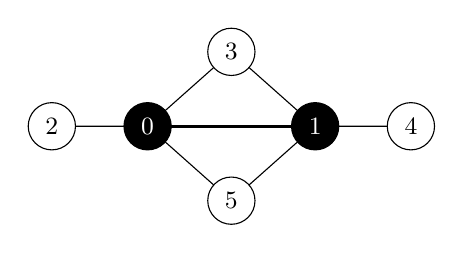
\begin{tikzpicture}[x=.95cm,y=.9cm,vertex/.style={draw=tinta,circle,fill=white,
minimum size=6mm,inner sep=0pt,font=\small}]
\coordinate (p0) at (-1.12,0); \coordinate (p1) at (1.12,0);
\coordinate (p2) at (-2.4,0); \coordinate (p4) at (2.4,0);
\coordinate (p3) at (0,1.05); \coordinate (p5) at (0,-1.05);
\draw[tinta] (p2)--(p0)--(p3)--(p1)--(p4) (p0)--(p5)--(p1);
\draw[rara,very thick] (p0)--(p1);
\foreach \i in {2,3,4,5}{\node[vertex] at (p\i) {\i};}
\foreach \i in {0,1}{\node[vertex,fill=tinta,text=white] at (p\i) {\i};}
\end{tikzpicture}

\small The set \(\{0,1\}\) is a vertex cover. Each \(e_i\) with \(i<7\) meets exactly one of these vertices.
\end{minipage}



\clearpage
\section{Optimal online value}
\begin{lema}\label{lem:on}
For the instance \(I_0\) of Section~\ref{sec:inst}, \(\ON(I_0)=80\).
\end{lema}
\begin{prueba}
Rejecting \(e_1,\ldots,e_6\) and accepting \(e_7\) when \(B_7=1\) yields expected reward \(\E[W_7]=80\). For the reverse inequality, fix an admissible policy \(\pi\). We may assume it rejects zero-weight edges. Indeed, one can simulate all its decisions internally and accept only the positive-weight edges it would accept. The actual matching is a subset of the simulated one and has the same weight on every realization.

Let \(T=\min\{i\leq6:A_i=1\}\), with \(T=\infty\) when this set is empty. For \(i\leq6\), the event \(\{T=i\}\) belongs to \(\F_i\) since it depends only on decisions through step \(i\). It is therefore independent of \((W_{i+1},\ldots,W_7)\). On \(\{T=i\}\), the first reward is \(w_i\), edge \(e_7\) is blocked, and all subsequent edges compatible with \(e_i\) meet the other vertex of the cover \(\{0,1\}\). At most one further edge can be accepted.

Let \(J_i\) be the ordered list of subsequent indices compatible with \(e_i\). For any such list, the optimal expected reward from a single selection satisfies
\[
 v(\varnothing)=0,\qquad
 v(j,J)=\E[\max\{W_j,v(J)\}].
\]
After observing \(W_j\), acceptance yields \(W_j\), whereas rejection leaves continuation value \(v(J)\) by independence. Backward induction gives an attainable maximum. Observing the weights of blocked edges or using a private seed leaves these continuation values unchanged. The six possible first acceptances give the following values.
\begin{center}
\begin{tabular}{@{}cclcl@{}}\toprule
\(i\)& \(J_i\)&Evaluation of \(v(J_i)\)& \(w_i\)& \(w_i+v(J_i)\)\\\midrule
1 & \((2,3,4)\)& \(\max\{44,33,60(3/4)\}=45\)&35&80\\
2 & \((5)\)& \(80(9/20)=36\)&44&80\\
3 & \((5,6)\)& \(80(9/20)+20(11/20)=47\)&33&80\\
4 & \((6)\)& \(80(1/4)=20\)&60&80\\
5, 6 & \(\varnothing\)& \(0\)&80&80\\\bottomrule
\end{tabular}
\end{center}
Hence \(\E[R_\pi(I_0)\mathbf 1_{\{T=i\}}]\leq80\,\Pr(T=i)\) for every \(i\leq6\). On \(\{T=\infty\}\), the reward is at most \(W_7\). Since \(\{T=\infty\}\in\F_6\), independence gives
\[
 \E[R_\pi(I_0)\mathbf 1_{\{T=\infty\}}]\leq
 \E[W_7]\Pr(T=\infty)=80\Pr(T=\infty).
\]
Summing over this partition gives \(\E[R_\pi(I_0)]\leq80\). The filtration includes the private seed from the outset, so this argument covers randomized policies.
\end{prueba}

\clearpage
\section{Offline optimum and proof of the theorem}
\begin{lema}\label{lem:off}
For the instance \(I_0\), \(\E[\OPT(I_0)]=\numoff/\masa\).
\end{lema}
\begin{prueba}
If \(B_7=1\), the prophet takes \(e_7\). Any matching omitting it has at most two edges, by the vertex cover \(\{0,1\}\), and weighs at most \(160\). Now suppose \(B_7=0\) and write \((a,b,c)=(B_4,B_5,B_6)\). Apart from \(e_7\), the edges at vertex 0 are \(e_2,e_3,e_4\), and those at vertex 1 are \(e_1,e_5,e_6\). The only incompatible pairs across the two groups are \((e_2,e_6)\) and \((e_4,e_5)\). Each single edge can be extended by a compatible edge from the other group. Since weights are nonnegative, the optimum is the maximum weight of a compatible pair:
\[
 H(a,b,c)=\max\left\{
 \begin{aligned}
 &44+\max\{35,80b\},\\
 &33+\max\{35,80b,80c\},\\
 &60a+\max\{35,80c\}
 \end{aligned}\right\}.
\]
Let \(q_{abc}=\Pr((B_4,B_5,B_6)=(a,b,c)\mid B_7=0)\). By independence this is the product of the three corresponding Bernoulli probabilities.
\begin{center}\renewcommand{\arraystretch}{1.14}
\begin{tabular}{@{}ccc@{\qquad}ccc@{}}\toprule
\(a\)&\(b\)&\(c\)&\(q_{abc}\)& Optimal pair & \(H(a,b,c)\)\\\midrule
0&0&0&\(33/320\)&\(e_1,e_2\)&79\\
0&0&1&\(11/320\)&\(e_3,e_6\)&113\\
0&1&0&\(27/320\)&\(e_2,e_5\)&124\\
0&1&1&\(9/320\)&\(e_2,e_5\)&124\\
1&0&0&\(99/320\)&\(e_1,e_4\)&95\\
1&0&1&\(33/320\)&\(e_4,e_6\)&140\\
1&1&0&\(81/320\)&\(e_2,e_5\)&124\\
1&1&1&\(27/320\)&\(e_4,e_6\)&140\\\bottomrule
\end{tabular}\end{center}


Summing the eight contributions gives
\(\sum_{a,b,c}q_{abc}H(a,b,c)=36\,163/320\). The law of total expectation yields
\[
 \E[\OPT(I_0)]
   =10^{-6}(80\,000\,000)+(1-10^{-6})\,\frac{36\,163}{320}
   =\frac{\numoff}{\masa}.
\]
\end{prueba}

\begin{prueba}[Proof of Theorem~\ref{thm:main}]
The construction in Section~\ref{sec:inst} satisfies the model assumptions. Lemmas~\ref{lem:on} and~\ref{lem:off} give the two identities. Evaluating the infimum defining \(c^\star\) at \(I_0\) gives
\[
 c^\star\leq\frac{\ON(I_0)}{\E[\OPT(I_0)]}
 =\frac{80\cdot\masa}{\numoff}
 =\frac{\numon}{\numoff}<\frac{41\,449}{100\,000}.
\]
The strict inequality follows by cross-multiplication of positive integers.
\end{prueba}

\clearpage
\section{Lean 4 certificate}
The formalization scales each expectation by \(\masa\) to work with integers. The lemma \texttt{policy\_le} proves by induction that the Bellman recurrence bounds the payoff of every policy that acts on the observed history. For the offline computation, the program enumerates weight realizations and then maximizes over feasible matchings separately for each realization.

{\raggedright The lemmas \texttt{witness\_online} and \texttt{witness\_offline} certify the respective numerators \(\numon\) and \(\numoff\). The theorem \texttt{universal\_upper} bounds rational guarantees. The lemma \texttt{private\_coins\_upper} gives the averaging step for a private random seed. The file imports only \texttt{Std} and can be checked with \texttt{lean ProphetMatchingWitness.lean}.\par}


\section{Related work and scope of the literature search}
Ezra et al.~\cite{ezra} distinguish vertex arrivals from edge arrivals. They establish the tight factor \(1/2\) for vertex arrivals and a guarantee of \(0.337\) for edge arrivals in general graphs. MacRury, Ma, and Grammel~\cite{mmg} improve the latter guarantee to \(0.344\). Together with Theorem~\ref{thm:main}, this gives
\[
 0.344 \;\leq\; c^\star \;\leq\; \frac{\numon}{\numoff}.
\]

Soto and Verdugo~\cite[Theorem~1(b)]{sv} prove the upper bound \(0.418928\) against the same integral offline optimum. Their construction also reserves a rare, high-value edge for the last arrival. Changing the preceding edges, their distributions, and their order gives a strictly smaller ratio here with a fixed positive probability for the final edge.

The \(4/11\) bound in their Theorem~1(a) concerns auctions in which one agent may value several edges. The \(0.390\) bound of Ma, MacRury, and Nuti~\cite{mmn} limits the \emph{selectability} of online contention resolution schemes (OCRSs), a per-edge requirement. This impossibility result alone does not upper-bound all policies measured against \(\E[\OPT]\). MacRury, Nuti, and Vondr\'ak~\cite{mnv} study matchoids, a broader class, and a fractional ex-ante benchmark.

\paragraph{Literature search (November 25, 2026).}
The search used the title and identifiers of~\cite{sv} and combinations of \emph{prophet matching}, \emph{edge arrivals}, \emph{upper bound}, and \emph{adversarial order}. At the time of the search, \href{https://openalex.org/W4409264837}{OpenAlex} grouped the preprint and journal article in one record with zero indexed citations. The search also screened titles citing~\cite{ezra} or~\cite{mmg} since October 16, 2024 (26 and 6 records respectively, with possible overlap), and examined relevant primary sources. The smallest published upper bound located for the model in Section~\ref{sec:modelo} was \(0.418928\). Index coverage limits any claim of priority.

\begingroup\small
\phantomsection\addcontentsline{toc}{section}{References}
\begin{thebibliography}{5}\setlength{\itemsep}{2pt}
\bibitem{ezra} T. Ezra, M. Feldman, N. Gravin and Z. G. Tang.
\href{https://doi.org/10.1287/moor.2021.1152}{Prophet Matching with General Arrivals}.
\emph{Mathematics of Operations Research} 47 (2022), 878--898.
\bibitem{sv} J. A. Soto and V. Verdugo.
\href{https://doi.org/10.1016/j.orl.2025.107294}{Prophet upper bounds for online matching and auctions}.
\emph{Operations Research Letters} 61 (2025), 107294. \href{https://arxiv.org/html/2410.12756v1#S3}{Proof of Theorem~1}.
\bibitem{mmg} C. MacRury, W. Ma and N. Grammel.
\href{https://doi.org/10.1137/1.9781611977554.ch76}{On (Random-order) Online Contention Resolution Schemes for the Matching Polytope of (Bipartite) Graphs}.
\emph{SODA} (2023).
\bibitem{mmn} W. Ma, C. MacRury and P. Nuti.
\href{https://arxiv.org/abs/2406.14506v3}{Online Matching and Contention Resolution for Edge Arrivals with Vanishing Probabilities}.
arXiv:2406.14506v3 (2026).
\bibitem{mnv} C. MacRury, P. Nuti and J. Vondrák.
\href{https://arxiv.org/abs/2609.20939}{Prophet Inequalities and Online Contention Resolution for Matchoids}.
arXiv:2609.20939 (2026).
\end{thebibliography}
\endgroup
\end{document}
